\section{moeo\-IBMOLS$<$ MOEOT, Move $>$ Class Template Reference}
\label{classmoeoIBMOLS}\index{moeoIBMOLS@{moeoIBMOLS}}
Indicator-Based Multi-Objective Local Search (IBMOLS) as described in Basseur M., Burke K.  


{\tt \#include $<$moeo\-IBMOLS.h$>$}

Inheritance diagram for moeo\-IBMOLS$<$ MOEOT, Move $>$::\begin{figure}[H]
\begin{center}
\leavevmode
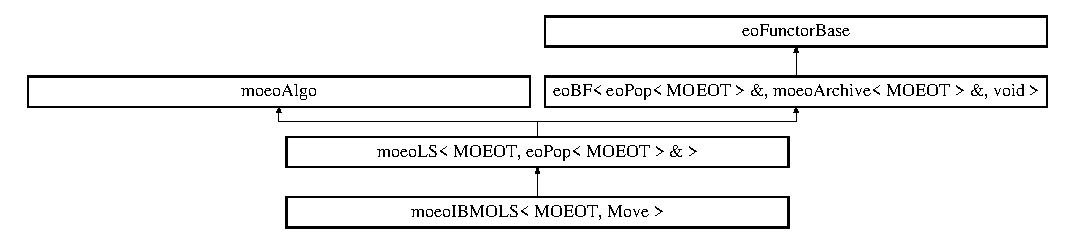
\includegraphics[height=2.83544cm]{classmoeoIBMOLS}
\end{center}
\end{figure}
\subsection*{Public Types}
\begin{CompactItemize}
\item 
typedef MOEOT::Objective\-Vector \bf{Objective\-Vector}\label{classmoeoIBMOLS_d3433001dcc9a6e2a967aa5d64163935}

\begin{CompactList}\small\item\em The type of objective vector. \item\end{CompactList}\end{CompactItemize}
\subsection*{Public Member Functions}
\begin{CompactItemize}
\item 
\bf{moeo\-IBMOLS} (mo\-Move\-Init$<$ Move $>$ \&\_\-move\-Init, mo\-Next\-Move$<$ Move $>$ \&\_\-next\-Move, \bf{eo\-Eval\-Func}$<$ MOEOT $>$ \&\_\-eval, \bf{moeo\-Move\-Incr\-Eval}$<$ Move $>$ \&\_\-move\-Incr\-Eval, \bf{moeo\-Indicator\-Based\-Fitness\-Assignment}$<$ MOEOT $>$ \&\_\-fitness\-Assignment, \bf{eo\-Continue}$<$ MOEOT $>$ \&\_\-continuator)
\begin{CompactList}\small\item\em Ctor. \item\end{CompactList}\item 
void \bf{operator()} (\bf{eo\-Pop}$<$ MOEOT $>$ \&\_\-pop, \bf{moeo\-Archive}$<$ MOEOT $>$ \&\_\-arch)
\begin{CompactList}\small\item\em Apply the local search until a local archive does not change or another stopping criteria is met and update the archive \_\-arch with new non-dominated solutions. \item\end{CompactList}\end{CompactItemize}
\subsection*{Private Member Functions}
\begin{CompactItemize}
\item 
void \bf{one\-Step} (\bf{eo\-Pop}$<$ MOEOT $>$ \&\_\-pop)
\begin{CompactList}\small\item\em Apply one step of the local search to the population \_\-pop. \item\end{CompactList}\end{CompactItemize}
\subsection*{Private Attributes}
\begin{CompactItemize}
\item 
mo\-Move\-Init$<$ Move $>$ \& \bf{move\-Init}\label{classmoeoIBMOLS_b4b4908b893edd52d6fa24085d2a89e5}

\begin{CompactList}\small\item\em the move initializer \item\end{CompactList}\item 
mo\-Next\-Move$<$ Move $>$ \& \bf{next\-Move}\label{classmoeoIBMOLS_8b8ebbd6eb6c82caa796160b4be2a86b}

\begin{CompactList}\small\item\em the neighborhood explorer \item\end{CompactList}\item 
\bf{eo\-Eval\-Func}$<$ MOEOT $>$ \& \bf{eval}\label{classmoeoIBMOLS_e9acda4b2f61f8960109a8c6fd52551e}

\begin{CompactList}\small\item\em the full evaluation \item\end{CompactList}\item 
\bf{moeo\-Move\-Incr\-Eval}$<$ Move $>$ \& \bf{move\-Incr\-Eval}\label{classmoeoIBMOLS_6c38636061bd03c4be809277e2dc257a}

\begin{CompactList}\small\item\em the incremental evaluation \item\end{CompactList}\item 
\bf{moeo\-Indicator\-Based\-Fitness\-Assignment}$<$ MOEOT $>$ \& \bf{fitness\-Assignment}\label{classmoeoIBMOLS_f48840d7af306db440e74028ed736a95}

\begin{CompactList}\small\item\em the fitness assignment strategy \item\end{CompactList}\item 
\bf{eo\-Continue}$<$ MOEOT $>$ \& \bf{continuator}\label{classmoeoIBMOLS_c15985c0bb5d9ba835f35d99d7c42b14}

\begin{CompactList}\small\item\em the stopping criteria \item\end{CompactList}\end{CompactItemize}


\subsection{Detailed Description}
\subsubsection*{template$<$class MOEOT, class Move$>$ class moeo\-IBMOLS$<$ MOEOT, Move $>$}

Indicator-Based Multi-Objective Local Search (IBMOLS) as described in Basseur M., Burke K. 

: \char`\"{}Indicator-Based Multi-Objective Local Search\char`\"{} (2007). 



Definition at line 32 of file moeo\-IBMOLS.h.

\subsection{Constructor \& Destructor Documentation}
\index{moeoIBMOLS@{moeo\-IBMOLS}!moeoIBMOLS@{moeoIBMOLS}}
\index{moeoIBMOLS@{moeoIBMOLS}!moeoIBMOLS@{moeo\-IBMOLS}}
\subsubsection{\setlength{\rightskip}{0pt plus 5cm}template$<$class MOEOT, class Move$>$ \bf{moeo\-IBMOLS}$<$ MOEOT, Move $>$::\bf{moeo\-IBMOLS} (mo\-Move\-Init$<$ Move $>$ \& {\em \_\-move\-Init}, mo\-Next\-Move$<$ Move $>$ \& {\em \_\-next\-Move}, \bf{eo\-Eval\-Func}$<$ MOEOT $>$ \& {\em \_\-eval}, \bf{moeo\-Move\-Incr\-Eval}$<$ Move $>$ \& {\em \_\-move\-Incr\-Eval}, \bf{moeo\-Indicator\-Based\-Fitness\-Assignment}$<$ MOEOT $>$ \& {\em \_\-fitness\-Assignment}, \bf{eo\-Continue}$<$ MOEOT $>$ \& {\em \_\-continuator})\hspace{0.3cm}{\tt  [inline]}}\label{classmoeoIBMOLS_04a4c1b453fe5ba2e3d44572196161fb}


Ctor. 

\begin{Desc}
\item[Parameters:]
\begin{description}
\item[{\em \_\-move\-Init}]the move initializer \item[{\em \_\-next\-Move}]the neighborhood explorer \item[{\em \_\-eval}]the full evaluation \item[{\em \_\-move\-Incr\-Eval}]the incremental evaluation \item[{\em \_\-fitness\-Assignment}]the fitness assignment strategy \item[{\em \_\-continuator}]the stopping criteria \end{description}
\end{Desc}


Definition at line 49 of file moeo\-IBMOLS.h.

\subsection{Member Function Documentation}
\index{moeoIBMOLS@{moeo\-IBMOLS}!operator()@{operator()}}
\index{operator()@{operator()}!moeoIBMOLS@{moeo\-IBMOLS}}
\subsubsection{\setlength{\rightskip}{0pt plus 5cm}template$<$class MOEOT, class Move$>$ void \bf{moeo\-IBMOLS}$<$ MOEOT, Move $>$::operator() (\bf{eo\-Pop}$<$ MOEOT $>$ \& {\em \_\-pop}, \bf{moeo\-Archive}$<$ MOEOT $>$ \& {\em \_\-arch})\hspace{0.3cm}{\tt  [inline, virtual]}}\label{classmoeoIBMOLS_fd788bbc4f956dec932dba2a4d4479b6}


Apply the local search until a local archive does not change or another stopping criteria is met and update the archive \_\-arch with new non-dominated solutions. 

\begin{Desc}
\item[Parameters:]
\begin{description}
\item[{\em \_\-pop}]the initial population \item[{\em \_\-arch}]the (updated) archive \end{description}
\end{Desc}


Implements \bf{eo\-BF$<$ eo\-Pop$<$ MOEOT $>$ \&, moeo\-Archive$<$ MOEOT $>$ \&, void $>$}.

Definition at line 72 of file moeo\-IBMOLS.h.

References moeo\-IBMOLS$<$ MOEOT, Move $>$::continuator, moeo\-Archive$<$ MOEOT $>$::equals(), moeo\-IBMOLS$<$ MOEOT, Move $>$::fitness\-Assignment, moeo\-IBMOLS$<$ MOEOT, Move $>$::one\-Step(), and moeo\-Archive$<$ MOEOT $>$::update().\index{moeoIBMOLS@{moeo\-IBMOLS}!oneStep@{oneStep}}
\index{oneStep@{oneStep}!moeoIBMOLS@{moeo\-IBMOLS}}
\subsubsection{\setlength{\rightskip}{0pt plus 5cm}template$<$class MOEOT, class Move$>$ void \bf{moeo\-IBMOLS}$<$ MOEOT, Move $>$::one\-Step (\bf{eo\-Pop}$<$ MOEOT $>$ \& {\em \_\-pop})\hspace{0.3cm}{\tt  [inline, private]}}\label{classmoeoIBMOLS_fce770398602972b5d67c52638687d43}


Apply one step of the local search to the population \_\-pop. 

\begin{Desc}
\item[Parameters:]
\begin{description}
\item[{\em \_\-pop}]the population \end{description}
\end{Desc}


Definition at line 119 of file moeo\-IBMOLS.h.

References moeo\-IBMOLS$<$ MOEOT, Move $>$::continuator, moeo\-IBMOLS$<$ MOEOT, Move $>$::fitness\-Assignment, moeo\-IBMOLS$<$ MOEOT, Move $>$::move\-Incr\-Eval, moeo\-IBMOLS$<$ MOEOT, Move $>$::move\-Init, and moeo\-IBMOLS$<$ MOEOT, Move $>$::next\-Move.

Referenced by moeo\-IBMOLS$<$ MOEOT, Move $>$::operator()().

The documentation for this class was generated from the following file:\begin{CompactItemize}
\item 
moeo\-IBMOLS.h\end{CompactItemize}
